\documentclass{classrep}
\usepackage[utf8]{inputenc}
\usepackage{polski}
\frenchspacing

\usepackage{graphicx}
\usepackage{amssymb}
\usepackage[usenames,dvipsnames]{color}
\usepackage[hidelinks]{hyperref}
\usepackage{float}

%new
\usepackage{amsmath, amssymb, mathtools}
\usepackage{fancyhdr, lastpage}
\pagestyle{fancyplain}
\fancyhf{}
\renewcommand{\headrulewidth}{0pt}
\definecolor{red}{rgb}{1, 0, 0}
\newcommand{\Csh}{C{\lserif\#}}

\studycycle{Informatyka, studia dzienne, I st.}
\coursesemester{VII}

\coursename{Technologie symulacji komputerowych}
\courseyear{2019/2020}

\courseteacher{dr. inż. Jan Rogowski}
\coursegroup{wtorek, 16:00}

\author{%
  \studentinfo[210347@edu.p.lodz.pl]{Krzysztof Wierzbicki}{210347}\\
  \studentinfo[210209@edu.p.lodz.pl]{Bartosz Jurczewski}{210209}%
}

\title{Zadanie: Symulacja płytki Chladniego }

\begin{document}
\maketitle
\thispagestyle{fancyplain}

\newpage

\section{Wstęp}
Zadaniem tworzonej przez nas aplikacji i modelu jest badanie drgań stalowej płytki wykonanej ze sprężystego materiału. \\
W symulacji zmianie będą mogły podlegać takie parametry jak: precyzja symulacji, postać drgań własnych, pozycja osi X i Y.

\section{Opis układu}
Symulacja układu będzie odbywać się w przestrzeni dwuwymiarowej, gdzie będziemy badać naprężenia występujące w stalowej płytce. 

\section{Opis obiektów biorących udział w symulacji}
W naszej symulacji możemy wyróżnić jeden główny obiekt będący fundamentem zagadnienia które chcemy symulować. Jest to wprawiona w drgania stalowa płyta. Zakładamy, że jest ona wykonana z materiału o kształcie płaskiego kwadratu, długość boku którego jest parametrem wejściowym symulacji.

Drgania własne dwuwymiarowej membrany można opisać równaniem falowym Bernoulliego
\begin{equation}
\frac{\partial^2 \Psi}{\partial t^2} = c^2 \Delta \Psi,
\end{equation}
gdzie $\Delta = \frac{\partial^2}{\partial x^2} + \frac{\partial^2}{\partial y^2}$, czyli Laplasjan po współrzędnych w rozważanej przestrzeni $\Omega \subset \mathbb{R}^2$, oraz $c$ jest stałą rzeczywistą określającą prędkość rozchodzenia się fali w ośrodku.
Falę stojącą w dwuwymiarowej przestrzeni $\Omega$ można opisać równaniem
\begin{equation}
\Psi(t, x, y) = v(t) \cdot u(x, y),
\end{equation}
gdzie funkcja $v(t) = A\cos{\omega t} + B\sin{\omega t}$ opisuje zmianę stanu w czasie, a $u(x, y)$ opisuje zależność amplitudy od położenia w przestrzeni i nazywana jest postacią drgań własnych (\textit{eigenmode}).
Możemy sprowadzić nasze rozważania do problemu poszukiwania wartości własnych przekształcenia Laplace'a. Korzystając z definicji problemu warunków brzegowych Dirichleta rozważamy równanie 
\begin{equation}
\Delta u +\lambda u=0
\end{equation}
z dodatnią stałą $\lambda$. %nie pytaj skąd to równanie, \lambda to wartość własna przekształcenia \Delta
Formułując ten problem jako zagadnienie rachunku wariacyjnego, po rozbiciu rozważanej powierzchni na siatkę trójkątów, będziemy mogli skorzystać z metody elementów skończonych aby rozwiązać równanie opisujące zbiór wartości i wektorów własnych 
\begin{equation} \label{big_integral}
\mathcal{I} = \frac{1}{2}\iint_\Omega \left(\left(\partial_x u\right)^2+\left(\partial_y u\right)^2-\lambda u^2\right)\mathrm{d}x\mathrm{d}y+\frac{1}{2}\int_{\partial \Omega} u^2\mathrm{d}s,
\end{equation}
gdzie $\partial\Omega$ oznacza krawędź dla której określone są warunki brzegowe. Jeżeli krawędź jest nieruchoma lub wolna, można odrzucić tę część równania.

Przedstawimy rozważaną przestrzeń $\Omega$ jako sumę trójkątów
\begin{equation}
\Omega \approx \bigcup_{i=1}^N T_i, \quad T_i = \triangle P_{i_1} P_{i_2} P_{i_3},
\end{equation}
gdzie $i_1, i_2, i_3$ -- indeksy punktów będących wierzchołkami $i$--tego trójkąta. Rozważana przez nas przestrzeń $\Omega$ jest kwadratem o boku długości $m$ jednostek. Wybierzemy $N = 2(m-1)^2$ trójkątów o wierzchołkach w punktach
\begin{equation}
P_{i_1}=(k+1, q), \quad P_{i_2}=(k, q), \quad P_{i_3}=(k+1, q+1)
\end{equation}
oraz
\begin{equation}
P_{i_1}=(k, q+1), \quad P_{i_2}=(k+1, q+1), \quad P_{i_3}=(k, q),
\end{equation}
otrzymując po $\frac{N}{2}$ trójkątów kolejno "górnych" i "dolnych" (będziemy indeksować trójkąty od $i=1$ tak, aby trójkąty "górne" miały indeksy parzyste, a trójkąty dolne indeksy nieparzyste).
Możemy wtedy przedstawić funkcję $u$ jako sumę funkcji wielomianowych będących przybliżeniem $u$ w dziedzinie odpowiadającej kolejnym trójkątom siatki
\begin{equation}
u(x, y) \approx \sum_{i=1}^N u_i(x, y).
\end{equation}
Przyjęcie tego założenia pozwala nam rozdzielić całkę przedstawioną w równaniu (\ref{big_integral}) na $N$ całek $\mathcal{I}_i$ odpowiadających kolejnym trójkątom. 
Dla $i$--tego trójkąta przeprowadzamy normalizację przekształcając współrzędne tak, aby punkty będące wierzchołkami trójkąta leżały na osiach współrzędnych, co ułatwi późniejsze obliczenia
\begin{equation}
x = 
\begin{cases}
x & \text{jeżeli $i$ jest nieparzyste}\\
-x & \text{w pozostałych przypadkach}
\end{cases}
\end{equation}
\begin{equation}
y = 
\begin{cases}
y & \text{jeżeli $i$ jest nieparzyste}\\
-y & \text{w pozostałych przypadkach}
\end{cases}
\end{equation}
Pochodne $i$--tej funkcji składowej $u_i$ przyjmują postać
Całka po $i$--tym trójkącie ma postać
\begin{equation} \label{other_big_integral}
2\mathcal{I}_i = 
\iint_{T_i} \left(\frac{\partial u_i}{\partial x}\right)^2 \mathrm{d}x\mathrm{d}y + 
\iint_{T_i} \left(\frac{\partial u_i}{\partial y}\right)^2 \mathrm{d}x\mathrm{d}y + 
\lambda \iint_{T_i} u_i^2 \mathrm{d}x\mathrm{d}y,
\end{equation}
Zakładając postać funkcji $u_i(x, y) = a_i + b_i x + c_i y$ i obliczając powyższe całki możemy sprowadzić wyrażenie (\ref{other_big_integral}) do postaci 
\begin{equation}
4\mathcal{I}_i = \Vec{u_i}^T
\begin{pmatrix}
0 & 0 & 0 \\
0 & 1 & 0 \\
0 & 0 & 0 \\
\end{pmatrix} 
\Vec{u_i} + \Vec{u_i}^T
\begin{pmatrix}
0 & 0 & 0 \\
0 & 0 & 0 \\
0 & 0 & 1 \\
\end{pmatrix}
\Vec{u_i} + \frac{1}{12}\lambda\Vec{u_i}^T
\begin{pmatrix}
12& 4 & 4 \\
4 & 2 & 1 \\
4 & 1 & 2 \\
\end{pmatrix}
\Vec{u_i}
\end{equation}
gdzie $\Vec{u_i} = (u_{i_1}, u_{i_2}, u_{i_3})$ $u_{i_j}$ oraz $u_{i_j}$ jest wartością funkcji $u_i$ w $j$--tym wierzchołku $i$--tego trójkąta.
Ostatecznie dla trójkąta $T_i$ możemy zapisać równanie
\begin{equation}
4\mathcal{I}_i = \Vec{u_i}^T (S_i - \lambda M_i) \Vec{u_i},
\end{equation}
gdzie 
\begin{equation}
S_i = 
\begin{pmatrix}
0 & 0 & 0 \\
0 & 1 & 0 \\
0 & 0 & 0 \\
\end{pmatrix}
+
\begin{pmatrix}
0 & 0 & 0 \\
0 & 0 & 0 \\
0 & 0 & 1 \\
\end{pmatrix}
=
\begin{pmatrix}
0 & 0 & 0 \\
0 & 1 & 0 \\
0 & 0 & 1 \\
\end{pmatrix}
\end{equation} nazywamy macierzą sztywności $i$--tego elementu, a 
\begin{equation}
M_i = 
\begin{pmatrix}
12& 4 & 4 \\
4 & 2 & 1 \\
4 & 1 & 2 \\
\end{pmatrix}
\end{equation}
nazywamy macierzą masy $i$--tego elementu.

Następnie należy złożyć macierze sztywności i masy poszczególnych elementów w macierze całego układu $\mathcal{S}$ oraz $\mathcal{M}$ rozmiaru $N \times N$. Zapiszemy też poszukiwane wartości funkcji $u$ w kolejnych wierzchołkach w postaci wektora kolumnowego $\Vec{u} = (u_1, u_2, ..., u_N)^T$. Początkowo macierze $\mathcal{S}$ i $\mathcal{M}$ inicjalizowane są wartościami $0$. Następnie dla kolejnych trójkątów $T_i$ z indeksami wierzchołków $(i_1, i_2, i_3)$ wykonujemy poniższe działania:
\begin{equation}
\mathcal{S}_{i_n i_m} += (S_i)_{nm}, \quad \mathcal{M}_{i_n i_m} += (M_i)_{nm}, \quad n, m \in \{1, 2, 3\}.
\end{equation}
Następnie usuwamy rzędy i kolumny odpowiadające nieruchomym punktom -- znamy wartości amplitudy w tych punktach. Ostatnim krokiem jest poszukiwanie ekstremów uzyskanego funkcjonału, $\delta \mathcal{I} = 0$, co prowadzi nas do układu wartości własnych
\begin{equation}
\mathcal{S}\Vec{u} = \lambda \mathcal{M}\Vec{u},
\end{equation}
który musi zostać rozwiązany. Dla każdej wartości własnej $\lambda$ wektor własny $\Vec{u}$ określa amplitudę na wszystkich wierzchołkach siatki.

\section{Uproszczenia}
W naszym modelu i symulacji przyjęliśmy kilka następujących uproszczeń:
\begin{itemize}
	\item Brak oporów ruchu.
	\item W rozpatrywanym przez nas przypadku materiał z którego wykonana jest rozpatrywana płyta jest jednorodny oraz izotropowy -- jego gęstość jest taka sama w każdym punkcie, a moduł Younga jest niezależny od kierunku.
	\item Parametry wejściowe symulacji można zmieniać podawać w zakresach przyjętych przez nas i zamieszczonych w tym sprawozdaniu.
\end{itemize}

\section{Środowisko i biblioteka graficzna}
Program zostanie zrealizowany za pomocą języka Python 3.8.0.

\section{Program}
Poniżej przedstawiamy screeny z naszego programu.
Parametry wejściowe:
\begin{itemize}
    \item Precision - dokładność
    \item Eigenmode number - postać drgań własnych
    \item X position - pozycja na osi X
    \item Y position - pozycja na osi Y
\end{itemize}

\begin{figure}[H]
	\centering
	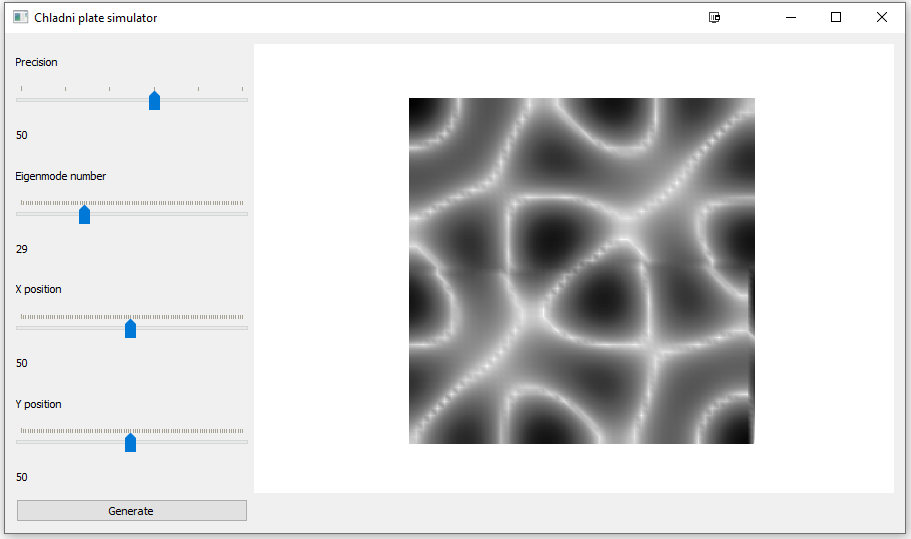
\includegraphics[width=1\textwidth]{{images/program_gui.png}}
	\caption{Widok programu}
\end{figure}

Dokładność rozumiemy jako ilość pikseli która składa się na bok kwadratu - wizualizacji.
\textcolor{red}{Nasz program obsługuje tylko te symulacje dla których wartość własna jest mniejsza od 0.5.}

\section{Wizualizacje}
Poniżej przedstawiamy uzyskane przez nas wizualizacje dla płytki o dokładności 50. Wartości pod rysunkami reprezentują postać drgań własnych.

\begin{figure}[H]
	\centering
	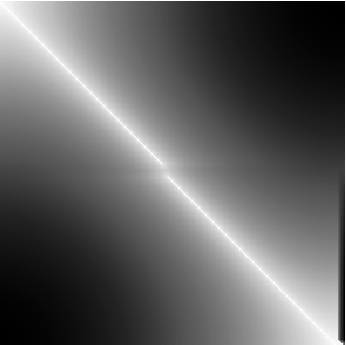
\includegraphics[width=0.48\textwidth]{{images/n1.png}}
	\caption{Postać drgań własnych: 1}
\end{figure}
\begin{figure}[H]
	\centering
	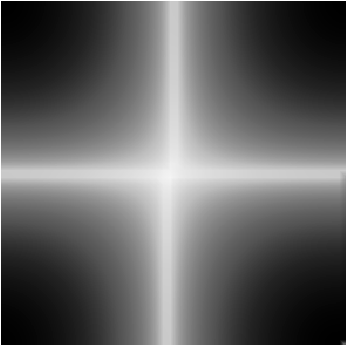
\includegraphics[width=0.48\textwidth]{{images/n3.png}}
	\caption{Postać drgań własnych: 3}
\end{figure}
\begin{figure}[H]
	\centering
	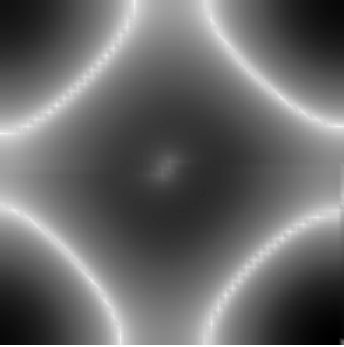
\includegraphics[width=0.47\textwidth]{{images/n5.png}}
	\caption{Postać drgań własnych: 5}
\end{figure}
\begin{figure}[H]
	\centering
	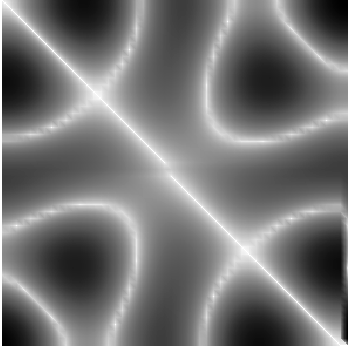
\includegraphics[width=0.47\textwidth]{{images/n17.png}}
	\caption{Postać drgań własnych: 17}
\end{figure}
\begin{figure}[H]
	\centering
	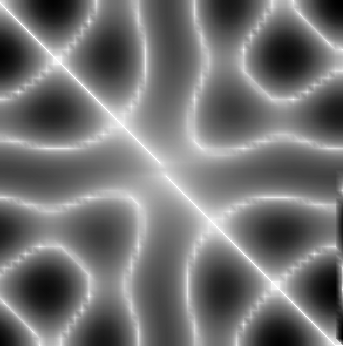
\includegraphics[width=0.47\textwidth]{{images/n35.png}}
	\caption{Postać drgań własnych: 35}
\end{figure}
\begin{figure}[H]
	\centering
	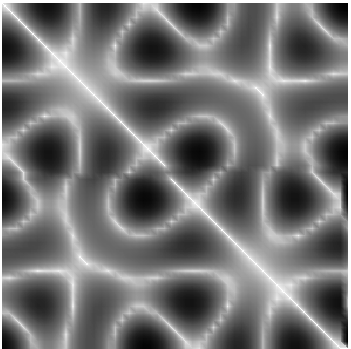
\includegraphics[width=0.47\textwidth]{{images/n50.png}}
	\caption{Postać drgań własnych: 50}
\end{figure}
\begin{figure}[H]
	\centering
	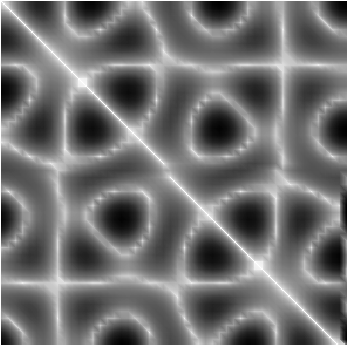
\includegraphics[width=0.47\textwidth]{{images/n65.png}}
	\caption{Postać drgań własnych: 65}
\end{figure}
\begin{figure}[H]
	\centering
	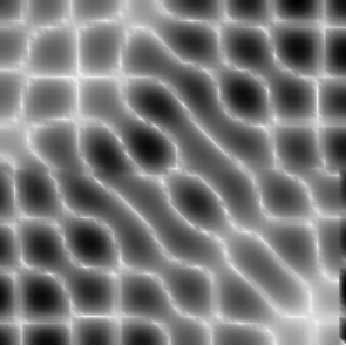
\includegraphics[width=0.47\textwidth]{{images/n85.png}}
	\caption{Postać drgań własnych: 85}
\end{figure}
\begin{figure}[H]
	\centering
	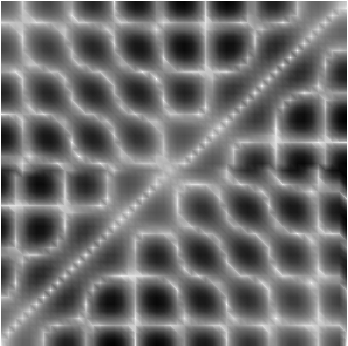
\includegraphics[width=0.47\textwidth]{{images/n99.png}}
	\caption{Postać drgań własnych: 99}
\end{figure}

\begin{thebibliography}{0}
  \bibitem{l2short} T. Oetiker, H. Partl, I. Hyna, E. Schlegl.
    \textsl{Nie za krótkie wprowadzenie do systemu \LaTeX2e}, 2007, dostępny
    online.
  \bibitem{numerical} T. Müller
    \textsl{Numerical Chladni figures}, 2013, \url{https://arxiv.org/pdf/1308.5523.pdf}
\end{thebibliography}

\end{document}
